\documentclass{article}
\usepackage{graphicx}

\title{Implementacja algorytmów RL oraz kontrolera rozmytego w środowisku highway-fast-v0}
\author{Damian Rogalski}
\date{June 2024}

\begin{document}

\maketitle

\section{Założenia projektowe}
\paragraph{}
Założeniem projektu była implementacja trzech algorytmów uczenia przez wzmacnianie tj. DQN, DQN+CNN, PPO oraz próba zaimplementowania sprawnie działającego kontrolera rozmytego do kontroli nad pojazdem w złożonym środowisku highway-fast-v0 z biblioteki Highway-env. Do implementacji algorytmu DQN, DQN+CNN oraz PPO skorzystałem z biblioteki stable baselines 3, natomiast do stworzenia kontrolera rozmytego skorzystałem z scikit-fuzzy.

\section{Środowisko highway-fast-v0}
\paragraph{}
Środowisko z biblioteki Highway-env, w którym celem jest poruszanie pojazdem w taki sposób, żeby rozwinął jak najwyższą predkość, za co otrzymuje najwyższą nagrodę, lecz za każdą kolizję otrzymuje karę. Na drodze znajdują się przeszkody w postaci innych pojazdów, które poruszają się z różną prędkością i potrafią zmieniać pasy. Kluczem jest wyuczenie własnego modelu manewru przyspieszania, hamowania, wyprzedzania innych pojazdów oraz zmiany toru jazdy.
Poniższa grafika przedstawia wygląd środowiska, zielony pojazd to samochód, którym steruje nasz algorytm, natomiast niebieskie pojazdy to nasze przeszkody.

\paragraph{}
\includegraphics[width=1\linewidth]{env.png}

\newpage


\section{Modele}
\subsection{DQN}
\paragraph{}
 Trenowanie modelu przeprowadziłem na 20 tysiącach epizodów gry. Początkowo model trenowałem stosując środowisko gymnasium uruchamiając go dla jednego procesu. Proces uczenia trwał 2 godziny i poskutkował utworzeniem przeuczonego modelu, który nie był skuteczny w dostosowywaniu się do zmieniających się warunków środowiska. Zamiast wykonywać optymalne manewry to zawsze decydował się zmienić pas na prawy i jechał po nim do końca często uderzając przy tym w poprzedzający pojazd, co całkowicie przekreślało sens jego wykorzystania. Postanowiłem wykorzystać sztuczne środowisko wektorowe uruchamiając w nim środowisko highway-fast-v0 dla 6 procesów jednocześnie. Pozwoliło to skrócić czas uczenia z 2 godzin do 3 minut. Wynikowy model nie jest przeuczony i cechuje się wyższą skutecznością w zmiennym środowisku. Przy procesie uczenia wykonałem również wykres osiągnietej nagrody dla konkretnego epizodu danego procesu. Oznacza to że oś X będzie przedstawiać liczbę wszystkich epizodów podzieloną przez liczbę procesów.


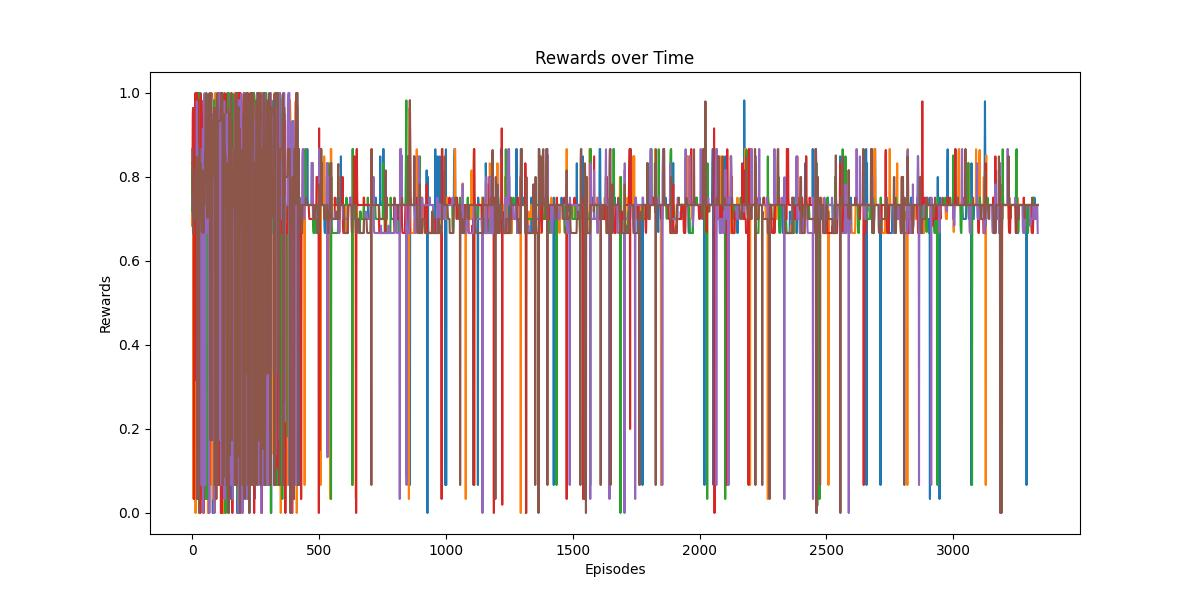
\includegraphics[width=1\linewidth]{DQN.jpg}
\paragraph{}
Wykres ukazuje przez wysoki rozrzut wyników, że model przez pierwsze 3000 epizdów nie radził sobie z predykcją właściwych akcji na bazie obserwacji środowiska, lecz kolejne epizody ukazują, iż model skuteczniej przewidywał akcje koncentrując swoje wyniki osiąganej nagrody około 0.7.

\newpage

\subsection{DQN+CNN}
\paragraph{}
Do trenowania modelu wykorzystałem środowisko z obserwacją ustawioną na skalę szarości. Uczenie przeprowadziłem na 100 tysiącach epizodów gry. Algorytm wyciąga obrazy i wykorzystuje je do uczenia się predykcji optymalnych zachowań. Korzystając z obliczanej nagrody określa, które zdjęcia przedstawiały najwyżej oceniane akcje. Do minimalizacji czasu wykorzystałem wektorowe środowisko uruchomione na jednym procesie. Trenowanie trwało przez 7 godzin i poskutkowało utworzeniem modelu o wysokiej skuteczności przewidywanych akcji niezależnie od stanu środowiska. Dla algorytm wykonałem wykres uczenia.


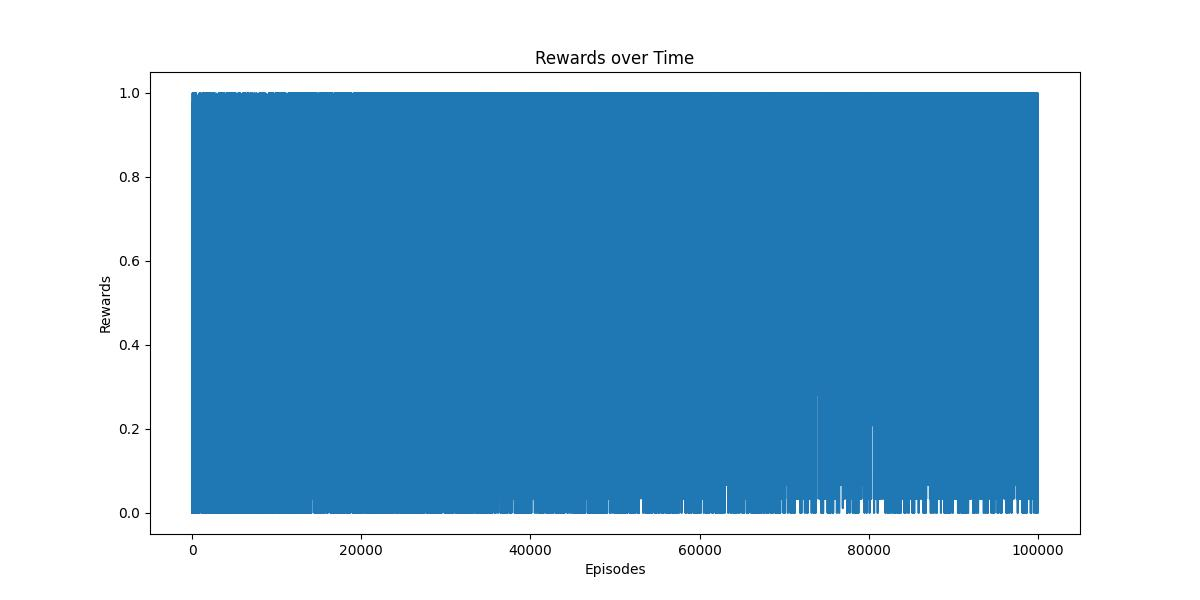
\includegraphics[width=1\linewidth]{DQN+CNN.jpg}
\paragraph{}
Wykres ukazuje że model przez cały cykl uczenia osiągał najwyższą nagrodę. Wynika to z faktu, że nagroda jest obliczana na podstawie uzyskanej prędkości maksymalnej, a algorytm od samego początku próbował sterować autem z najwyższą możliwą prędkością bez względu na ryzyko kolizji z innym pojazdem. Ostatnia ćwiartka epizodów pokazuje spadek niższych wyników osiąganych nagród, co wskazuje, że model zaczął bardziej rozważnie przewidywać akcje.

\newpage

\subsection{PPO}
\paragraph{}
Tak jak w przypadku DQN początkowo przeprowadziłem trenowanie w środowisku gymnasium dla 20 tysięcy epizodów, co zajęło 3 godziny i stworzyło przeuczony model, który miał niską skuteczność przewidywania ruchów i zachowywał się tak samo jak przeuczony model z algorytmem DQN. Stwierdziłem, że powtórzę proces trenowania w środowisku wektorowym na 6 procesach jednocześnie dla 20 tysięcy epizodów gry, który skrócił czas do 1 minuty. Wynikowy model osiąga podobną skuteczność, co DQN wymagając przy tym krótszego czasu trenowania przy takiej samej liczbie epizodów.


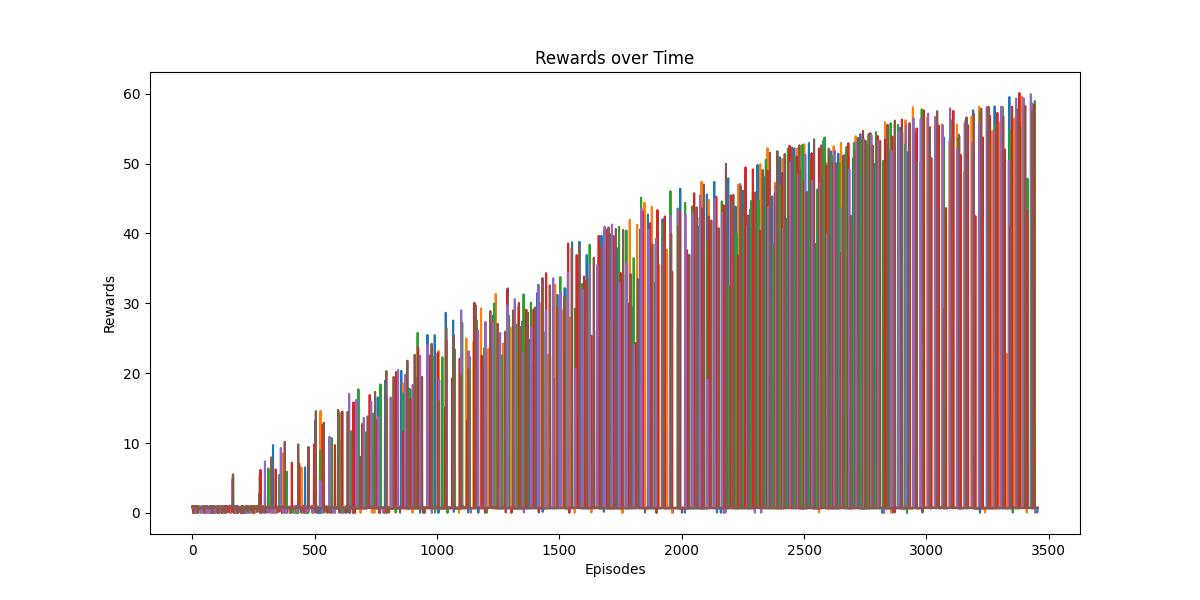
\includegraphics[width=1\linewidth]{PPO_20k_episodes.jpg}

\paragraph{}
Wykres pokazuje stabilny wzrost osiąganej nagrody względem kolejnych epizodów, gry. Wskazuje to, że model nie jest przeuczony.

\newpage

\paragraph{}
Wykonałem również kolejny trening modelu dla 100 tysięcy epizodów gry przy reszcie parametrów takich jak dla poprzedniego modelu.

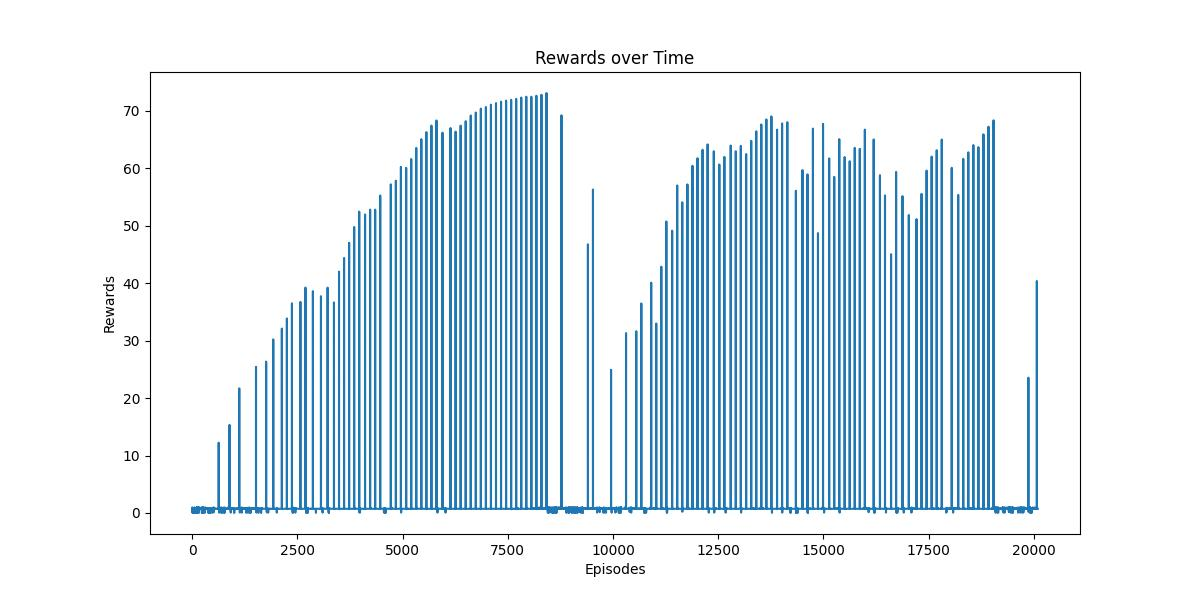
\includegraphics[width=1\linewidth]{PPO.jpg}

\paragraph{}
Wykres przedstawia, że model osiągnął wyższą maksymalną nagrodę w stosunku do swojego poprzednika. Do około 6000 epizodu każdego z procesów model uczył się w stabilnym tempie, jednakże przy kolejnych epizodach przestał, co wskazuje, że nie był w stanie znaleźć lepszej strategii bądź został przetrenowany.


\subsection{Kontroler rozmyty}
\paragraph{}
Moja implementacja kontrolera rozmytego zawiera zestaw pięciu zmiennych lingwistycznych dla odległości (very\_close, close, medium, far, very\_far), pięciu dla prędkości (very\_slow, slow, average, fast, very\_fast) oraz pięciu dla podejmowanych akcji (brake\_hard, brake, keep\_lane, change\_left, change\_right). Baza reguł zawiera 25 różnych możliwych akcji. Niestety przez skomplikowanie kontrolera i środowiska mój kontroler nie radzi sobie z właściwym dobieraniem akcji do warunków środowiska.

\newpage

\section{Podsumowanie}
\paragraph{}
Algorytmy uczenia przez wzmacnianie doskonale sprawdziły się w kontroli pojazdem w zmiennym środowisku. Najlepiej sprawdził się DQN+CNN, który potrafi rozwinąć najwyższą predkość i sprawnie radzi sobie z wyprzedzaniem innych pojazdów. DQN i PPO okazały się mniej skuteczne, gdyż nie potrafią rozwinąć tak wysokiej prędkości oraz rzadko próbują wyprzedzi auto przed sobą, jednakże z wysoką skutecznością gwarantują, że pojazd nie uderzy w inne samochody. Kontroler rozmyty nie sprawdził się w kontroli pojazdem z uwagi na wysokie skomplikowanie problemu. Pomimo wielu prób i zmian w jego logice nie był on w stanie w niezawodny sposób prawidłowo podejmować optymalne akcje.

\end{document}
